\documentclass[12pt,spanish]{article}
\usepackage[utf8]{inputenc}
\usepackage{babel}
\usepackage{listings}
\usepackage{mathpazo}
\usepackage{enumitem}
\usepackage{courier}
\usepackage{textcomp}
\usepackage{xcolor}
\usepackage{parskip}
\usepackage{fullpage}

\newcommand{\onelinerule}{\rule[2.3ex]{0pt}{0pt}}
\newcommand{\twolinerule}{\rule[6.2ex]{0pt}{0pt}}
\newcommand{\respuesta}{\framebox[\textwidth]{\twolinerule}}
\newcommand{\nombre}{%
  \begin{tikzpicture}[xscale=.4,yscale=.7]
    \draw (0, 0) rectangle (22, 1);
  \end{tikzpicture}%
}
%\newcommand{\rol}   {\framebox[0.3\textwidth]{\onelinerule}}
\newcommand{\rol}{%
  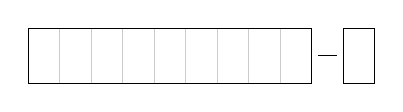
\begin{tikzpicture}[xscale=.4,yscale=.7]
    \draw[gray!40] ( 0, 0) grid      ( 9, 1);
    \draw          ( 0, 0) rectangle ( 9, 1);
    \draw          (10, 0) rectangle (11, 1);
    \draw (9 + .2, .5) -- (10 - .2, .5);
  \end{tikzpicture}%
}
\newcommand{\li}{\lstinline}
\providecommand{\pond}[1]{[{\small\textbf{#1\%}}]}

\lstdefinelanguage{py}{%
  classoffset=0,%
    morekeywords={%
      False,class,finally,is,return,None,continue,for,lambda,try,%
      True,def,from,nonlocal,while,and,del,global,not,with,print,%
      as,elif,if,or,yield,assert,else,import,pass,break,except,in,raise},%
    keywordstyle=\color{black!80}\bfseries,%
  classoffset=1,
    morekeywords={int,float,str,abs,len,raw_input,exit,range,min,max,%
      set,dict,tuple,list,bool,complex,round,sum,all,any,zip,map,filter,%
      sorted,reversed,dir,file,frozenset,open,%
      array,zeros,ones,arange,linspace,eye,diag,dot},
    keywordstyle=\color{black!50}\bfseries,%
  classoffset=0,%
  sensitive=true,%
  morecomment=[l]\#,%
  morestring=[b]',%
  morestring=[b]",%
  stringstyle=\em,%
}

\lstdefinelanguage{testcase}{%
  moredelim=[is][\bfseries]{`}{`},%
  backgroundcolor=\color{gray!20},%
}

\lstdefinelanguage{file}{%
  frame=single,%
}

\lstset{language=py}
\lstset{basicstyle=\ttfamily}
\lstset{columns=fixed}
\lstset{upquote=true}
\lstset{showstringspaces=false}
\lstset{rangeprefix=\#\ }
\lstset{includerangemarker=false}

\newlist{certamen}{enumerate}{1}
\setlist[certamen]{%
  label=\arabic*.,
  font=\LARGE\bfseries,%
  labelindent=-.5in,%
  leftmargin=0pt,%
  labelsep=1em%
}



\lstset{language=testcase,frame=single}

\begin{document}
  \thispagestyle{empty}
  \section*{Lunes 3 de septiembre}

  Los \emph {números de Fibonacci} son
  la siguiente sucesión de números enteros:
  \[
      0,   1,    1,    2,    3,
      5,   8,   13,   21,   34,
     55,  89,  144,  233,  377,
    610, 987, 1597, 2584, 4181, \ldots
  \]
  Los primeros términos de la sucesión son 0 y 1,
  y de ahí en adelante cada término es la suma de los dos anteriores.

  Escriba los siguientes programas:
  \begin{enumerate}[leftmargin=0pt]

    \item
      \begin{minipage}[t]{0.7\textwidth}
        \small
        \lstinputlisting[linerange=C1-FIN\ C1]{casos.txt}
      \end{minipage}

    \item
      \begin{minipage}[t]{0.7\textwidth}
        \small
        \lstinputlisting[linerange=C2-FIN\ C2]{casos.txt}
      \end{minipage}

    \item
      \begin{minipage}[t]{0.7\textwidth}
        \small
        \lstinputlisting[linerange=C3-FIN\ C3]{casos.txt}
      \end{minipage} \\
      \begin{minipage}[t]{0.7\textwidth}
        \small
        \lstinputlisting[linerange=C4-FIN\ C4]{casos.txt}
      \end{minipage}


  \end{enumerate}

\end{document}

